\documentclass[10pt,letterpaper,subeqn]{beamer}
\setbeamertemplate{navigation symbols}{}
\usefonttheme{serif}
\usecolortheme{orchid}



\usepackage[english]{babel}
\selectlanguage{english}
\usepackage{bm}
\usepackage{booktabs}
\usepackage{color}
\usepackage[update,prepend]{epstopdf}
\usepackage{framed}
\usepackage{fleqn}
\usepackage{graphics}
\usepackage{hyperref}
\usepackage[utf8]{inputenc}
\usepackage{setspace}
\usepackage{textcomp}
\usepackage{wrapfig}
\usepackage{multirow}
\usepackage{caption}
\usepackage{subcaption}
\setbeamertemplate{caption}[numbered]


\title{Assessing Plan B: The Effect of the Morning After Pill on Children and Women}
\author{Damian Clarke}
\institute{University of Oxford}
\date{June 2014}



\begin{document}


\begin{frame}
\titlepage
\end{frame}


\section{Introduction}
\frame{\frametitle{This Talk}
\begin{enumerate}
\item There was \textcolor{blue}{quasi-experimental} variation in 
\textcolor{blue}{morning after pill} availability in Chile.  
\item Availability \textcolor{blue}{reduced teenage childbearing} and (illegal) 
abortions by an important amount.
\item The control group may be partially treated via \textcolor{blue}{spillovers}.  
Propose a way to recover consistent estimates.
\end{enumerate}
}

\frame{\frametitle{Motivation}
\begin{itemize}
\item Considerable evidence that the oral contraceptive pill improves outcomes for women and children
\begin{itemize}
\item Delays in childbearing, marriage (Angrist and Evans, 1996)
\item Higher education, labour market participation (Goldin and Katz, 2002)
\item Reduction in gender wage differential (Bailey 2012)
\end{itemize}
\item But, \textcolor{blue}{scarce evidence on the effects of post-coital birth control}
\item A small number of papers from expansions in USA, nothing outside USA, nor at national level
\item Would like to know: how does the introduction of the ``morning after pill'' affect 
fertility/abortions?
\end{itemize}
}

\frame{\frametitle{Importance}
\begin{itemize}
\item Oral contraceptive pill provided fundamental change in ability to control total fertility and timing (Bailey 2006)
\item However, requires a costly, ongoing and regular investment
\item The morning after pill however, is a once-off contraceptive (non-abortive) treatment
\item In many situations it is much cheaper or fully subsidised
\item Also, non-abortive, so present in circumstances even where abortion is illegal
\item May operate at a different margin (younger women and women not regularly contracepting)
\end{itemize}
}

\frame{\frametitle{The Context}
A finding by the Supreme Court of Chile making the morning after pill legal, but at the
discretion of each mayor in local jurisdictions
\vspace{5mm}
\begin{itemize}
\item This is quite different to USA literature given that abortion is entirely outlawed in Chile
\item Previously, any person in Chile wanting to post coitally contracept had to:
\begin{itemize}
\item Risk illegal abortion which is prosecuted, dangerous and stigmatised; or
\item Have access to the information that high doses of the pill act similarly to the post-coital pill
\end{itemize}
\item High rates of teen pregnancy (48.60 per 1000 women aged 15-19 in 2012)
\item Low rates of contraceptive coverage (12.9\% of 15-19 year olds using any form)
\end{itemize}
}

\section{Methods}
\frame{\frametitle{Methodology}
\[
 \label{TEENeqn:pill}
birth_{ijt} = \alpha + \delta\cdot \mathbb{I}\{Pill_{jt-1}\} + \phi_t + \eta_j + 
\eta_j\cdot t + X_{jt-1}\gamma + \varepsilon_{ijt}.
\]
\vspace{5mm}
\begin{itemize}
\item Flexible diff-in-diffs
\item Woman $i$ in municipality $j$ and time $t$ is `treated' if public health
centres report that the pill is freely available upon request
\item Identifying assumption is parallel trends; pill placement is conditionally
exogenous
\end{itemize}
}

\frame{\frametitle{Estimating Treatment Effects in The Presence of Treatment Spillovers}
\[
y_{ijct} = \alpha + \delta\cdot \mathbb{I}\{Pill_{jt-1}\} + 
\sum_{c=0}^C\zeta_c\cdot close_{cdjt-1} + \hdots + \varepsilon_{ijct}
\]
where
\[
 close_{cdjt} =
  \begin{cases}
   1 & \text{if } dist_{jt} > c \wedge dist_{jt}\leq c+d   \\
   0 & \text{if } dist_{jt} \leq c \vee  dist_{jt}>c+d.
  \end{cases}
\]
\vspace{5mm}
\begin{itemize}
\item Test what happens if we exclude from the control group women `close to' the pill
\item Let the data determine who is `close' and who isn't
\item This loosens SUTVA, but still requires that this hold in non-close municipalities
\item Cluster errors to allow for spatial correlation (Conley, 1999)
\end{itemize}
}

\frame{\frametitle{General Identification Challenges}
Parallel trends assumption would be violated if pill and non-pill mayors simultaneously embark
on other related policies
\begin{itemize}
\item Selection into prescribing the pill is largely based on mayor's ideology, however not
necessarily along party lines
\item Pill law was passed mid-electoral cycle
\item Add a series of time-varying controls
\item Undertake a series of robustness checks using false (lagged) treatments
\end{itemize}
}

\section{Data}
\frame{\frametitle{The Reform}
Constitutional finding of the Supreme Court in 2008 regarding ``National Laws for the Regulation
of Fertility'' (Law 20.418)
\begin{itemize}
\item Made it legal for all Municipal Health Centres to distribute the EC pill freely to women
\item Of the 346 municipalities in Chile, approximately 150 immediately reported that they 
distribute the EC pill without restriction
\item EC pill prescriptions jumped sharply, from 0 in 2007 to approximately 7,000 doses in 2008
\end{itemize}
}

\frame{
\begin{figure}[htpb!]
\begin{center}
\caption{Pill Prescriptions and Availability by Time}
\label{TEENfig:Pilltime}
\vspace{-5mm}
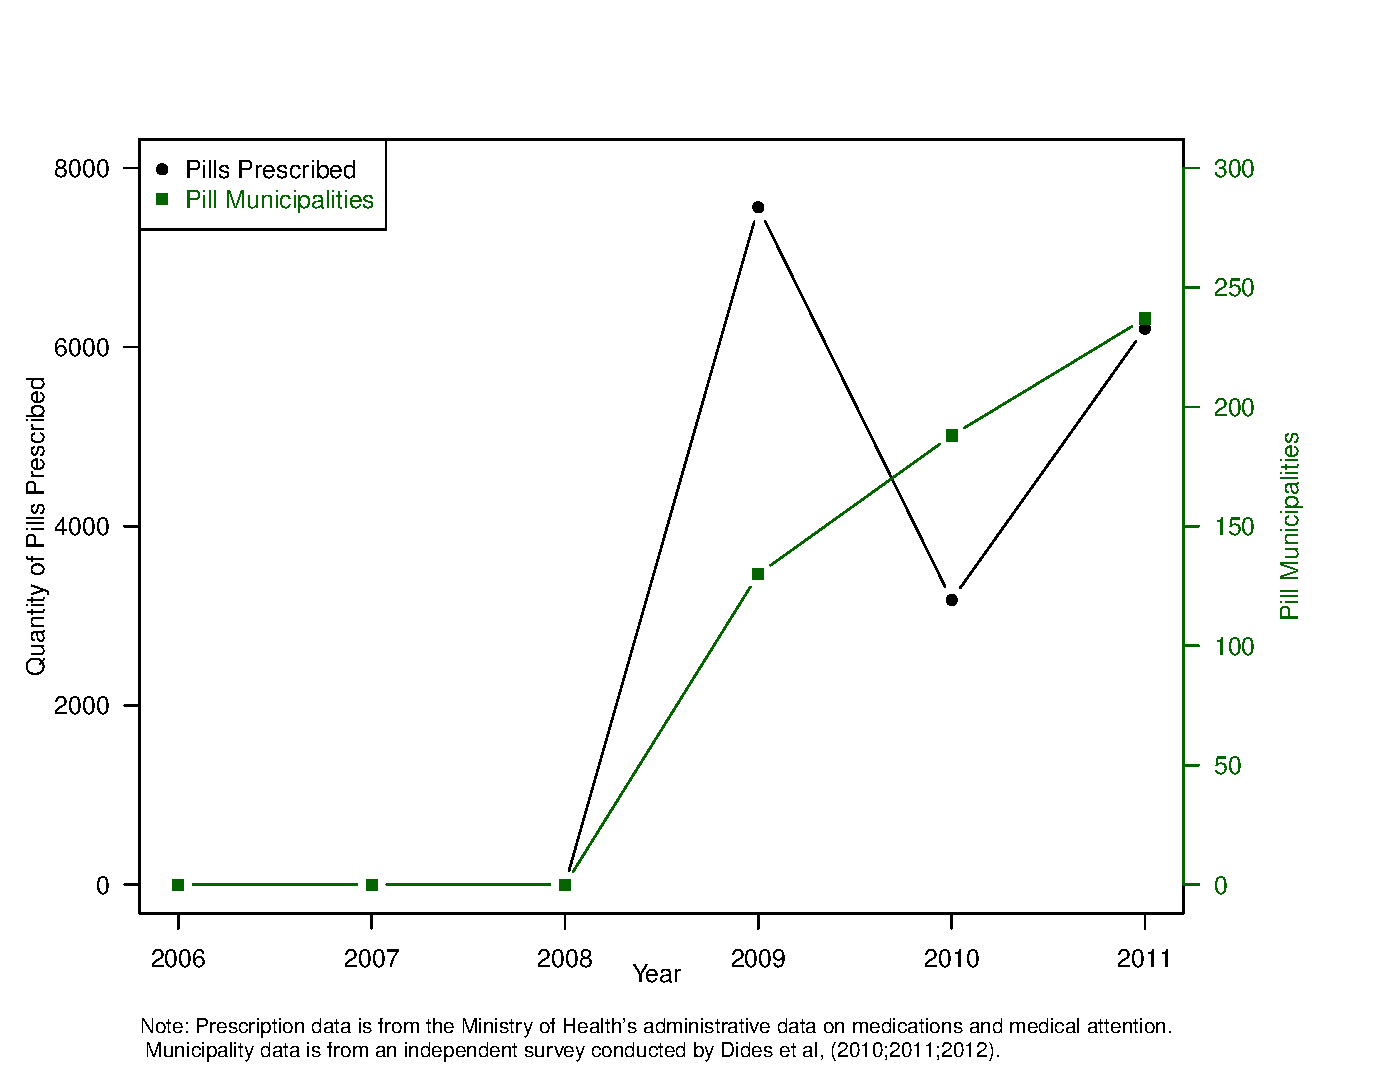
\includegraphics[scale=0.44]{./figures/Pill.eps} 
\end{center}
\end{figure}
}

\frame{
\begin{figure}[htpb!]
\begin{center}
\caption{The Availability of the Pill by Geographic Region}
\label{TEENfig:PillGeo}
\includegraphics[scale=0.2]{./figures/Pill_l.eps}
\end{center}
\end{figure}
}

\frame{\frametitle{Data}
\begin{itemize}
\item Matched administrative data files recording all live births and fetal deaths in Chile
\item Crossed with data recording population by municipality.  Principal outcomes:
\begin{itemize}
\item Births per woman
\item Fetal deaths per live birth (late term, early term)
\end{itemize}
\item All births and deaths from 2006--2011.  1,391,565 births; 11,387 fetal deaths
\item Measure of treatment comes from an independent survey (Dides et al.\ 2009, 2010, 2011)
\item Also have administrative data on pill disbursements
\end{itemize}
}




\frame{
\begin{figure}[htpb!]
\begin{center}
\caption{Total Recorded Births and Fetal Deaths, 2006-2011}
\label{TEENfig:BirthDeath}
\vspace{-5mm}
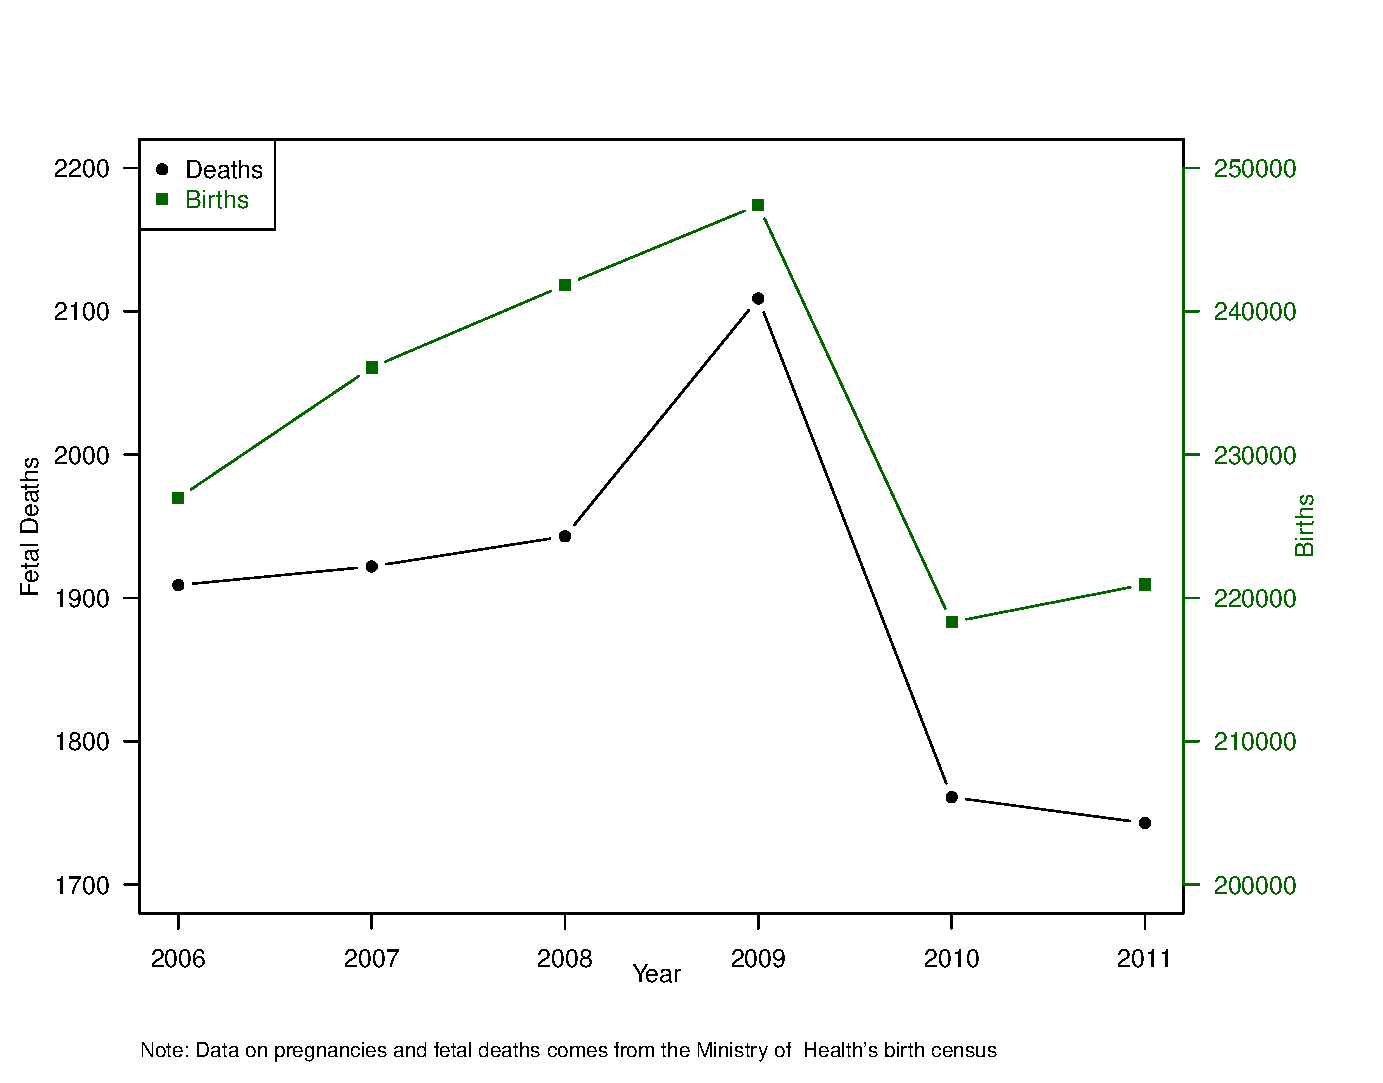
\includegraphics[scale=0.44]{./figures/BirthDeath.eps} 
\end{center}
\end{figure}
}

\section{Results}
\frame{\frametitle{Results}
Headline results:
\begin{itemize}
\item Naive estimates of the effect of having the morning after pill available:
\begin{itemize}
\item Reduces births by 5.5\% for teenagers
\item Reduces births by 3.7\% for 20-34 year olds
\item No effect on 35-44 year olds
\item Strong evidence for reduction in early term fetal deaths, no effect on late term
\end{itemize}
\item However, strong evidence of spillovers.  Those living `close to' pill municipalities 
also have:
\begin{itemize}
\item Reduction in births for 15--19, 20--34 year olds
\item Reduced rates of early-term fetal deaths
\item These effects persist for distances up to 30km\ldots
\end{itemize}
\end{itemize}
}

\frame{\frametitle{Births}
\begin{table}[!htbp] \centering
\caption{The Effect of the Morning After Pill on Pregnancy}
\label{TEENtab:PillPreg}
\scalebox{0.5}{
\begin{tabular}{@{\extracolsep{5pt}}lccccp{1mm}cccc}
\\[-1.8ex]\hline \hline \\[-1.8ex] 
&\multicolumn{4}{c}{All Births}&&\multicolumn{4}{c}{First Births}
\\ \cmidrule(r){2-5} \cmidrule(r){7-10}
&(1)&(2)&(3)&(4)&&(5)&(6)&(7)&(8)\\ \hline
\multicolumn{10}{l}{\textsc{\noindent 15-19 year olds}} \\
 & & & & & & & & & \\
Morning After Pill &$-$0.064$^{***}$&$-$0.065$^{***}$&$-$0.057$^{***}$&$-$0.057$^{***}$&&$-$0.036$^{**}$&$-$0.041$^{***}$&$-$0.031$^{**}$&$-$0.036$^{**}$\\
 &(0.015)&(0.015)&(0.015)&(0.015)&&(0.015)&(0.016)&(0.016)&(0.016)\\
 & & & & & & & & & \\
Observations&4,152,490&4,152,490&4,152,490&4,152,490&&4,125,336&4,125,336&4,125,336&4,125,336\\
McFadden's $R^2$&0.670&0.670&0.671&0.671&&0.633&0.634&0.635&0.636\\
 & & & & & & & & & \\
\multicolumn{10}{l}{\textsc{\noindent 20-34 year olds}} \\
 & & & & & & & & & \\
Morning After Pill &$-$0.040$^{***}$&$-$0.039$^{***}$&$-$0.038$^{***}$&$-$0.038$^{***}$&&$-$0.024$^{*}$&$-$0.029$^{**}$&$-$0.026$^{*}$&$-$0.029$^{**}$\\
 &(0.010)&(0.011)&(0.011)&(0.012)&&(0.014)&(0.014)&(0.015)&(0.015)\\
 & & & & & & & & & \\
Observations&11,022,111&11,022,111&11,022,111&11,022,111&&10,458,703&10,458,703&10,458,703&10,458,703\\
McFadden's $R^2$&0.772&0.772&0.773&0.773&&0.684&0.685&0.685&0.686\\
 & & & & & & & & & \\
\multicolumn{10}{l}{\textsc{\noindent 35-49 year olds}} \\
 & & & & & & & & & \\
Morning After Pill &0.001&0.001&0.005&0.008&&0.042&0.039&0.040&0.042\\
 &(0.013)&(0.013)&(0.013)&(0.013)&&(0.036)&(0.038)&(0.038)&(0.039)\\
 & & & & & & & & & \\
Observations&10,572,196&10,572,196&10,572,196&10,572,196&&10,376,895&10,376,895&10,376,895&10,376,895\\
McFadden's $R^2$&0.537&0.537&0.538&0.538&&0.641&0.641&0.642&0.642\\
\hline \\[-1.8ex] 
{\small Trends \& FEs} & Y & Y & Y & Y && Y & Y & Y & Y \\
{\small Political Controls} & & Y & Y & Y && & Y & Y & Y \\
{\small Health, Educ Controls} & & & Y & Y && & & Y & Y \\
{\small Gender Controls} & & & & Y && & & & Y \\
\hline \hline \\[-1.8ex]
\end{tabular}}\end{table}

}

\frame{\frametitle{Fetal Deaths}
\begin{table}[htpb!] \centering
\caption{The Effect of the Morning After Pill on Fetal Deaths}
\label{TEENtab:PillDeath}
\scalebox{0.5}{
\begin{tabular}{@{\extracolsep{5pt}}lccc}\\[-1.8ex]
\hline\hline\\[-1.8ex]
& All & Early & Late \\
& Deaths & Gestation & Gestation \\ 
& (1) & (2) & (3) \\ \midrule
\multicolumn{4}{l}{\textsc{15-19 year olds}} \\
&&&\\
Morning After Pill &$-$0.185$^{**}$&$-$0.815$^{***}$&$-$0.155\\
&(0.081)&(0.183)&(0.111)\\
&&&\\
Mean (deaths/live birth)&0.008&0.002&0.005\\
Observations&219,608&218,388&218,911\\
McFadden's $R^2$&0.232&0.378&0.251\\
&&&\\
\multicolumn{4}{l}{\textsc{20-34 year olds}} \\
&&&\\
Morning After Pill &$-$0.058&$-$0.189$^{*}$&$-$0.071\\
&(0.048)&(0.102)&(0.055)\\
&&&\\
Mean (deaths/live birth)&0.007&0.002&0.004\\
Observations&954,424&949,477&951,577\\
McFadden's $R^2$&0.198&0.385&0.170\\
&&&\\
\multicolumn{4}{l}{\textsc{35-49 year olds}} \\
&&&\\
Morning After Pill &$-$0.488$^{***}$&$-$0.776$^{***}$&$-$0.544$^{***}$\\
&(0.079)&(0.208)&(0.101)\\
&&&\\
Mean (deaths/live birth)&0.012&0.003&0.007\\
Observations&228,920&227,029&227,781\\
McFadden's $R^2$&0.260&0.411&0.238\\
\hline \hline \\[-1.8ex]
\end{tabular}}\end{table}

}

\frame{\frametitle{Spillovers}
\begin{table}[!htbp] \centering
\caption{The Morning After Pill and Treatment Spillovers}
\label{TEENtab:Spillover} 
\scalebox{0.64}{
\begin{tabular}
{@{\extracolsep{5pt}}lccc}\\[-1.8ex]\hline\hline\\
[-1.8ex] & 15-19 & 20-34 & 35-49 \\
& Year olds & Year olds & Year olds \\ \midrule
\multicolumn{4}{l}{\textsc{\noindent Panel A: Births}} \\
& & & \\
Morning After Pill &$-$0.071$^{***}$&$-$0.043$^{***}$&0.014\\
&(0.017)&(0.014)&(0.015)\\
Close $<15$ km &$-$0.077$^{***}$&$-$0.042$^{***}$&0.018\\
&(0.021)&(0.014)&(0.017)\\
Close 15-30 km &$-$0.057$^{**}$&$-$0.014&0.019\\
&(0.023)&(0.013)&(0.023)\\
Close 30-45 km &$-$0.037&$-$0.016&0.031\\
&(0.035)&(0.028)&(0.030)\\
& & & \\
Observations&4,152,490&11,022,111&7,117,890\\
McFadden's $R^2$&0.674&0.774&0.527\\ \midrule
\multicolumn{4}{l}{\textsc{\noindent Panel B: Fetal Deaths}}\\
&&&\\
Morning After Pill &$-$0.834$^{***}$&$-$0.175&$-$0.942$^{***}$\\
&(0.226)&(0.131)&(0.283)\\
Close $<15$ km &$-$0.154&$-$0.022&$-$0.200\\
&(0.235)&(0.151)&(0.240)\\
&&&\\
Observations&218,388&949,477&194,327\\
McFadden's $R^2$&0.380&0.386&0.417\\
\hline \hline \\[-1.8ex]
\multicolumn{4}{p{9.2cm}}{\begin{footnotesize}\textsc{Notes:}
$^{*}$p$<$0.1; $^{**}$p$<$0.05; $^{***}$p$<$0.01;\end{footnotesize}}
\normalsize\end{tabular}}\end{table}

}

\frame{
\begin{figure}[htpb!]
\begin{center}
\caption{Estimates of $\hat\delta^c$ for Pregnancy (15-19)}
\label{TEENfig:Dist1519}
\vspace{-5mm}
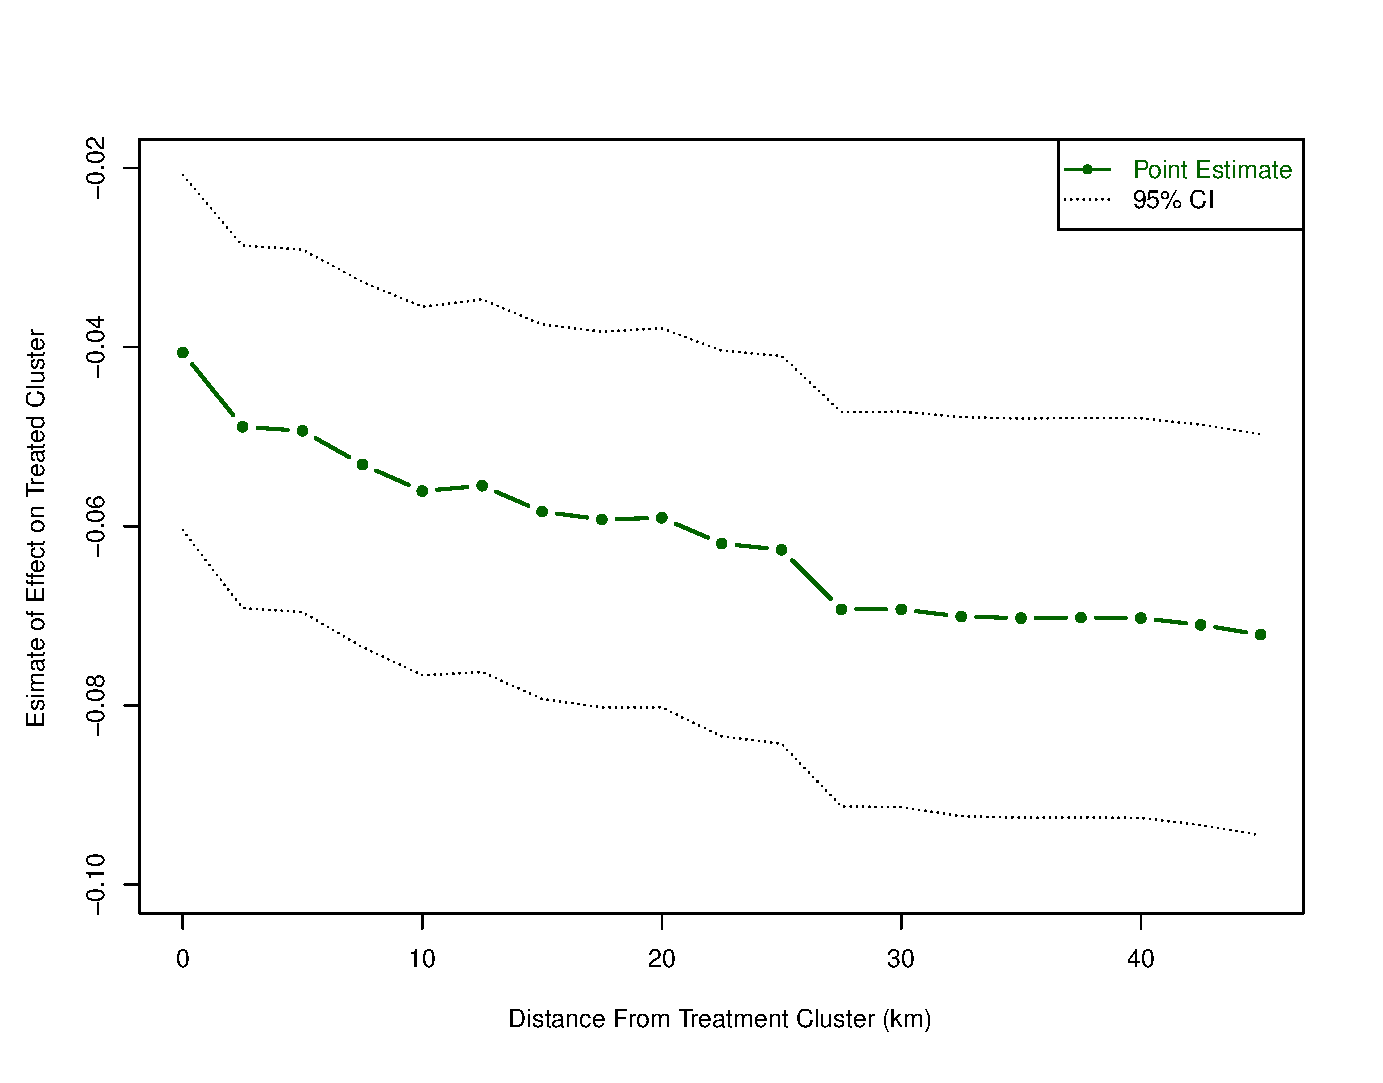
\includegraphics[scale=0.44]{./figures/Dist1519.eps} 
\end{center}
\end{figure}
}

\frame{\frametitle{Plausibility?}
These are large effects, and indeed much larger than what is reported in the two economic studies that exist in the USA.  However:
\begin{itemize}
\item These effects are smaller than the estimates of viewing ``16 and Pregnant'' [ADD LINK]
\item In Chile, prior to the morning after pill, outside options were very limited: either give birth, travel to abort, or risk death/incarceration in the country
\item In cases where abortion exists, this technology may shift women from abortion to post-coital contraceptives, and so may not turn up in net figures
\item A back of the envelope calculation suggests that the effectiveness of the pill (pregnancies avoided per prescription) is $\sim$0.7-0.8.  The US FDA suggests that typical use has effectiveness of 89\% [ADD LINK]
\end{itemize}
}


\section{Discussion}
\frame{\frametitle{The Take Away Points}
\begin{enumerate}
\item There was \textcolor{blue}{quasi-experimental} variation in 
\textcolor{blue}{morning after pill} availability in Chile.  
\item Availability \textcolor{blue}{reduced teenage childbearing} and (illegal) 
abortions by an important amount.
\item The control group may be partially treated via \textcolor{blue}{spillovers}.  
Propose a way to recover consistent estimates.
\end{enumerate}
}


\end{document}


%********************************************************************************
%********************************************************************************
%********************************************************************************
%********************************************************************************
%********************************************************************************
%********************************************************************************
%********************************************************************************
%********************************************************************************
%********************************************************************************
%********************************************************************************
